\begin{figure}[H]
    \centering
    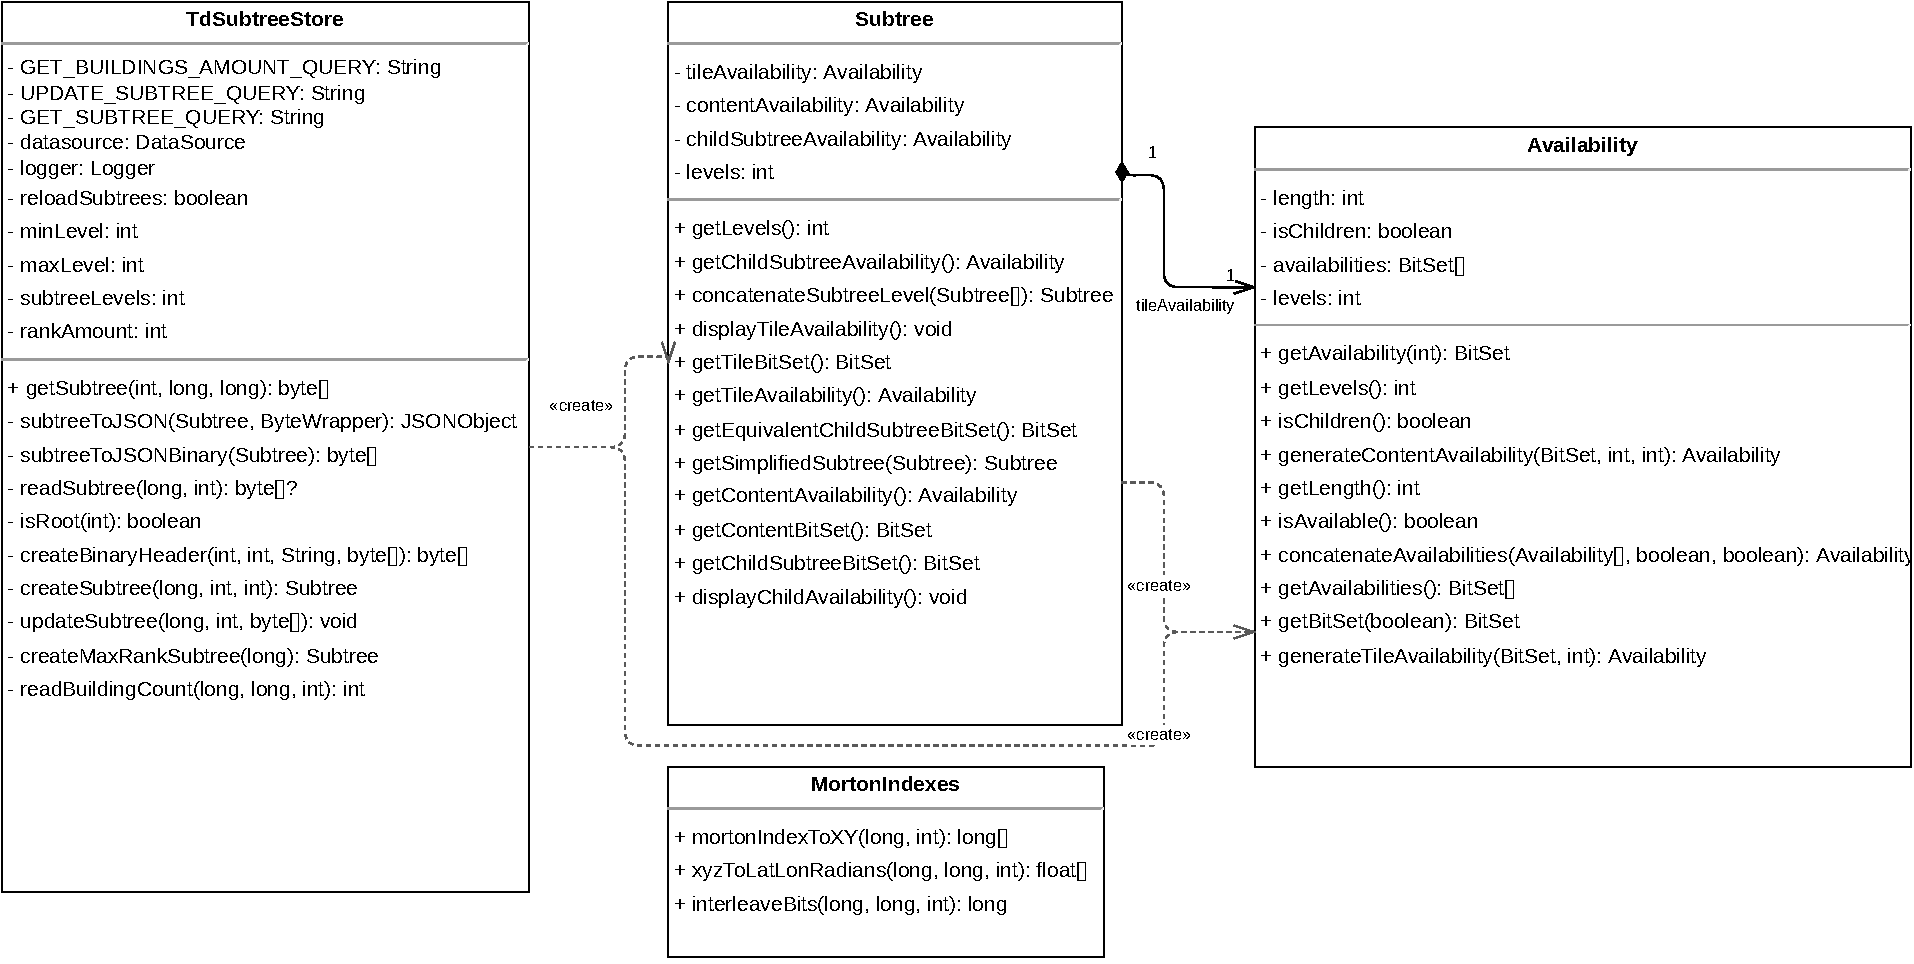
\includegraphics[width=1\textwidth]{assets/figures/subtree-classes.drawio.pdf}
    \caption{Classes utilisées pour la création d'une hiérarchie de Subtrees}
    \label{fig:subtree-classes}
\end{figure}

\subsection*{Classe Subtree\footnote{src/main/java/org/apache/baremaps/tdtiles/Subtree/Subtree.java}}
\label{sec:subtree-class}

La première classe écrite dans le but de gérer les Subtrees est la classe \texttt{Subtree}. Un objet de cette classe comporte tout les éléments nécessaires pour la gestion d'un Subtree. Il contient un objet \texttt{Availability} pour chaque type de disponibilité (tuile, contenu, enfants) ainsi que le nombre de levels contenu. La classe offre aussi tous les getters utiles pour accéder aux informations importantes. Elle fournit aussi une fonction statique de concaténation de 4 Subtrees en un d'ordre supérieur. Cette fonction sera utilisée pour la création de l'arbre de Subtrees. Finalement, elle offre deux fonction de debug pour afficher les \textit{Tile Availability} et le \textit{Child Availability} dans la console.

\subsection*{Classe Availability\footnote{src/main/java/org/apache/baremaps/tdtiles/Subtree/Availability.java}}
\label{sec:availability-class}

La classe Availability est celle qui se chargera de stocker les listes de disponibilités. Pour cela, elle utilise un \textit{BitSet} par soucis d'optimisation. Tout comme la classe Subtree, elle offre une fonction de concaténation de 4 \textit{Availability} en un seul. De plus, elle propose deux fonctions pour générer un Availability complet à partir d'un BitSet représentant le dernier level du Subtree.

Trois types de disponibilités sont possibles : tuile, contenu et enfants. La disponibilité des tuiles indique si une tuile peut être accédée par le client Cesium. La disponibilité des contenus indique si une tuile contient des bâtiments ou non. Pour finir, la disponibilité des enfants indique si un Subtree enfant au Subtree actuel à une \textit{root tile} (cf. \autoref{fig:subtree-hierarchy}) qui est disponible. Cette dernière information servira au client Cesium à savoir si il doit demander à l'API un Subtree enfant ou non.

Une liste de disponibilités est donc, comme précisé auparavant, une liste de boolean représentant un des trois types de disponibilité pour chaque tuile du Subtree. Cela veut dire qu'une seule liste de disponibilité s'occupe de tout les niveaux du Subtree. Ces listes de disponibilités sont en théorie stockées dans un seul Bitset qui comprend tous ces niveau. Dans mon implémentation, j'ai choisi de stocker chaque niveau dans un BitSet différent. Cela ne change rien car à l'envoi du Subtree au client, les BitSets seront concaténés dans un seul buffer binaire.

Pour comprendre comment les différents niveaux de tuiles sont représentées dans un BitSet, je vous invite à regarder la figure ci-dessous :

\begin{figure}[H]
    \centering
    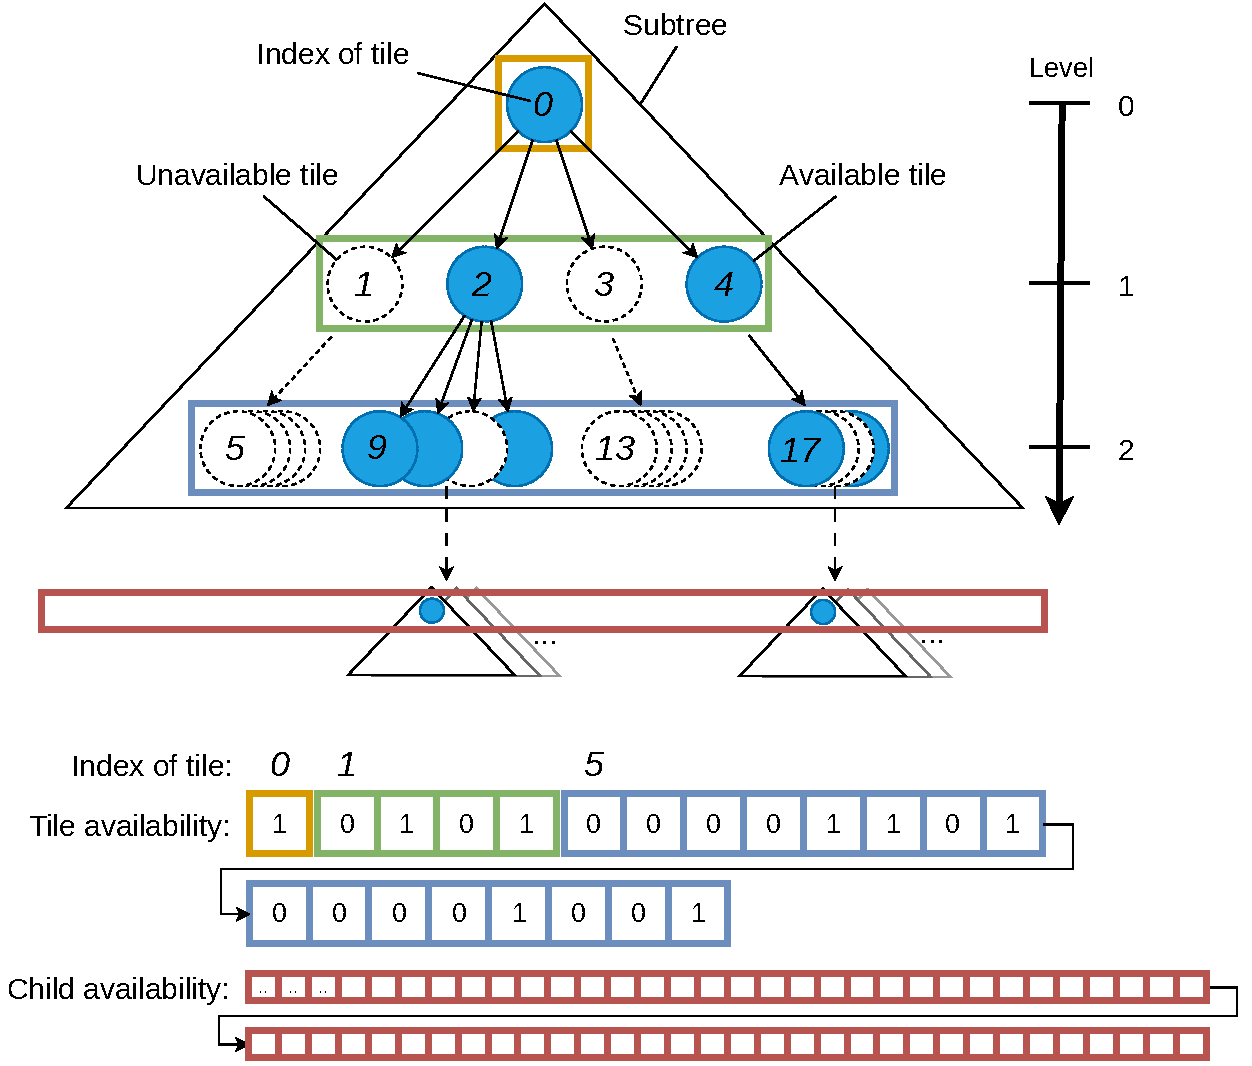
\includegraphics[width=1\textwidth]{assets/figures/availability-levels.drawio.pdf}
    \caption{Représentation des niveaux de tuiles dans un BitSet}
    \label{fig:availability-levels}
\end{figure}

Vous remarquerez que les listes de disponibilités n'ont pas toutes la même longueur. La longueur des listes de disponibilités des tuiles et des contenus suit la formule suivante :

\[
length = \frac{(4^{subtreeLevels} - 1)}{3} \text{avec} \quad subtreeLevels \quad \text{le nombre de niveaux d'un Subtree}
\]

La longueur des listes de disponibilités des enfants suit la formule suivante :

\[
length = 4^{subtreeLevels}
\]

Dans l'exemple de la \autoref{fig:availability-levels}, les Subtrees sont composés de 3 niveaux (\texttt{subtreeLevels}). Les listes de disponibilités des tuiles et des contenus auront donc une longueur de 21 et la liste de disponibilités des enfants aura une longueur de 64.

\newpage
\subsection*{Classe TdSubtreeStore\footnote{src/main/java/org/apache/baremaps/tdtiles/TdSubtreeStore.java}}
\label{sec:tdsubtreestore-class}

Cette classe est celle qui orchestrera la création et la distribution des Subtrees. Ce processus suit le diagramme suivant :

\begin{figure}[H]
    \centering
    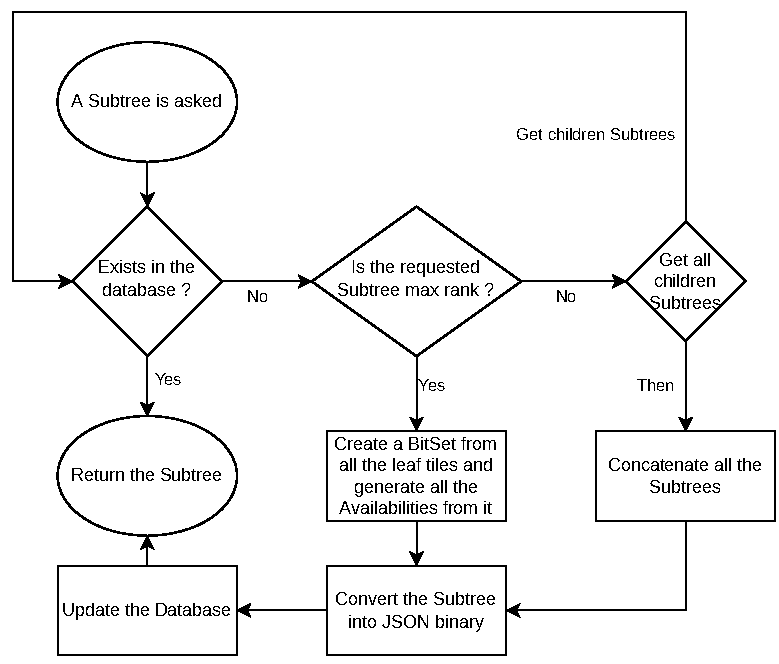
\includegraphics[width=1\textwidth]{assets/figures/simple-flowchart.drawio.pdf}
    \caption{Flowchart de la classe \texttt{TdSubtreeStore}}
    \label{fig:ssimple-flowchart}
\end{figure}

Vous observerez que la classe utilise un système récursif pour la création d'un Subtree. Puisqu'un Subtree parent doit être au courant des disponibilités des Subtrees enfants, il faudrait en théorie que ces derniers soient connus. Cependant, cela peut être optimisé en ne faisant que regarder si des bâtiments se trouvent dans la tuile enfant. Pour cela, une simple requête SQL simple permet de le déterminer :

\begin{verbatim}
SELECT EXISTS (
    SELECT 1
    FROM osm_ways
    WHERE (tags ? 'building' OR tags ? 'building:part')
    AND st_intersects(geom, st_makeenvelope(%1$s, %2$s, %3$s, %4$s, 4326))
) OR EXISTS (
    SELECT 1
    FROM osm_relations
    WHERE (tags ? 'building' OR tags ? 'building:part')
    AND st_intersects(geom, st_makeenvelope(%1$s, %2$s, %3$s, %4$s, 4326))
) AS has_buildings
\end{verbatim}

Les deux méthodes ont des avantages et des inconvénients. La méthode calculant tous les Subtrees est énormément plus lente, mais les utilisateurs n'auront pas de temps d'attente supplémentaire lorsqu'ils se déplaceront dans la carte. La méthode calculant les Subtrees au fur et à mesure est quasiment instantanée, mais les utilisateurs devront attendre un peu plus longtemps lorsqu'ils se déplaceront dans la carte pour la première fois.

Pour le développement de l'application, je recommande donc de ne pas calculer tous les Subtrees en avance car il y en a rarement besoins. Par contre, pour un usage en production, il serait préférable de les calculer en avance.

Ce choix ainsi que le choix de re-créer les Subtrees ou les fichiers glTF des tuiles peuvent être modifiés dans la classe \texttt{TdTilesResources}\footnote{src/main/java/org/apache/baremaps/server/TdTilesResources.java}.